
\documentclass[11pt]{article}
\usepackage[utf8]{inputenc}
\usepackage{fullpage}
\usepackage{times}
\usepackage{graphicx}
\usepackage{multicol}
\usepackage{amsmath}
\usepackage{tabularx}
\usepackage{setspace}
\raggedright

\renewcommand{\contentsname}{Innehållsförteckning}
\renewcommand{\figurename}{Figur}
\renewcommand{\tablename}{Tabell}

\begin{document}

% Frontpage
\begin{titlepage}

\begin{center}


\vspace*{4cm}

% Title
{ \huge \bfseries Core Wars}\\[0.2cm]
{ \Large \bfseries TSEA43}\\[0.2cm]
{ Projektrapport}\\[0.2cm]

\vspace*{2cm}

Jonas Hietala \\
Jesper Tingvall \\
Jizhi Li

\vfill

% Bottom of the page
{\large 7 Maj, 2012}

\end{center}

\end{titlepage}
\newpage

% empty after frontpage
\newpage
\thispagestyle{empty}
\mbox{}


% 2nd page
\newpage
\section*{Sammanfattning}

I detta projekt har vi byggt en mikrodator som använder Redcode som assembler. Detta för att kunna spela spelet Core Wars. Vi använder en UART för att skriva in koden till datorns minne och vi kan dumpa ut minnesinnehållet och spelets status på en skärm genom VGA-porten. I rapporten går vi igenom lite Redcode, beskrivning av hårdvara till vår mikrodator och hur vi använder RS232 och VGA standarden. Till sist har vi en del exempel Warriors som visar de vanligaste Core Wars strategierna.

\thispagestyle{empty}
\newpage


% 3rd page
\tableofcontents

\thispagestyle{empty}
\newpage


% 4th page. Start page numbering here.
\setcounter{page}{1}
\pagenumbering{arabic}

% Space up paragraphs a bit
\setlength{\parskip}{4mm plus1mm minus3mm}

\section{Inledning}

Vårt mål med projektet i denna TSEA43 kurs var att bygga en dator som kunde köra det eminenta spelet Core Wars. Core Wars är ett ointeraktivt spel där spelarna skriver sina program i Redcode assembler. Målet var att bygga en maskin som använde Redcode som sin assembler och som kunde måla ut spelområdet, d.v.s. minnet, till en VGA skärm och ta emot ny kod via en UART. För mer utförlig information om våra designmål rekommenderas en läsning i vår designskiss \footnote{Se bilaga TODO}.

Vi namnger vår dator till M.A.R.C, Memory Array Redcode Computer då simulatorn heter M.A.R.S, Memory Array Redcode Simulator. Värt att nämna är att Core Wars ej refererat till processor kärnan utan till ett gammalt kärnminne.

Vårt mål är att kunna spela Core Wars enligt 1988 standarden\footnote{http://corewars.nihilists.de/redcode-icws-88.pdf}, skicka in innehåll till M.A.R.C från en kontrolldator och sätta ut två spelares position. Vi vill även kunna dump ut minnesinnehåll och spelstatus till en VGA skärm. Vår uDator skall kunna utföra alla 10 instruktioner och 4 adresseringsmoder Redcode har samt kunna växla mellan, skapa och ta bort processer. Vi rekommenderar en läsning utav 1988 standarden då vi ej kommer att gå igenom instruktionerna eller adresseringsmoderna i denna rapport.

\newpage

% 5th page.
\section{ICWS88 Redcode}

\subsection{Introduktion}
Vi har programmerat en assembler som kan generera en binärfil ifrån två Warriors skrivna i Redcode. Vi randomiserar också deras startläge. Vi kan sedan skicka den assemblerade koden och startpositionerna till MARC genom UART.

\subsection{Exempel Warriors}

\textbf{Replicator} \\
Replicators skapar kopior av sig själva och förökar sig i minnet. De motverkar bombers då bombers inte kan förstöra replicatorn tillräckligt snabbt.

\textbf{Factory Bomber} \\
Factory bomber (eller bomber factory då den bygger bombers) formaterar hela minnet via att masskopiera en massa ’little bombers’ till minnet. Dessa databombar minnet och kommer efter ett tag bomba isär orginalkoden. Denna Warrior är därmed en blandning mellan en bombare och en replicator.

\textbf{Carpet Bomber} \\
Carpet bombers är en blandning mellan en bomber och en scanner. De traverserar minnet och lägger in bombers där minnet har ändrats. Denna Warrior är smartare än en vanlig bomber då den inte kommer att bomba ute i tomma minnet. Den kommer också vara lite snabbare än en traditionell bomber som behöver kopiera ut data.

\textbf{Imp Spawner} \\
Denna Warrior är ej offensiv och har som stategi att skapar en massa imps. Imp spawner fungerar ungefär som Factory Bomber fast har en annan payload.

\textbf{Vampire Bomber Gate Replicator} \\
Denna otympliga Warrior startade som ett skämt då vi ville se vad som hände om man inkluderade så många strategier som möjligt i en Warrior. Dock blev den inte så dålig som vi först trodde. Först så skapar Warriorn en kopia av sig själv, denna kopia kan dock ej kopiera sig själv, något som borde kunna lösas med hjälp av lite hjärnverksamhet och en texteditor. Efter kopiatorn så har Warriorn en ”bomber cage”, dessa två rader databombar minnet bakåt. Efter cagen kommer vampyrkoden. En vampyr JMP bombar minnet i hopp om att fienden skall hoppa in i dess cage. Den kan därmed sno klockcykler ifrån motståndarens kod. Sist finns en gate ifall resten av koden skulle bli överkörd av en Imp.

\textbf{Kopimi} \\
Denna Warrior scannar minnet efter information, kopierar den och börjar sen exekvera den. Den kan därmed härma en fientlig Warrior om den skulle hitta den. Fungerar skapligt trots att den utvecklades mest för att se vad som hände om man skulle tolka Det Missionerande Kopimistsamfundet missionsbudskap\footnote{http://kopimistsamfundet.se}; ”Kopiera och sprid” i form av Redcode. Denna Warrior använder replicator strategin.

\textbf{Inseminator} \\
Ännu en Warrior som skapades på skoj men som visade sig vara rätt så effektiv. Den letar upp motståndarens kod och injicerar en massa processer i den i hopp om att motståndaren ej ska förstöra sig egen kod. Detta brukar dock förstöra funktionaliteten i motståndarens kod då den förutsätter oftast att koden exekveras sekventiellt.

\textbf{Core Cleaner} \\
En core cleaner är ett program som databombar hela minnet. Ofta går man igenom minnet två gånger, den första fyller man minnet med split instruktioner för att slöa ner motståndaren och sedan med DAT-instruktioner för att göra slut på honom.

\textbf{Dwarf Scout} \\
En dwarf scout är en enkel bomber som skyddar sig mot andra bombers genom att se om någon ändrar i minnet i dess närhet. Om så är fallet så kommer den att hoppa till en ny plats i minnet och ta med sig sina processer.

\newpage

\section{Teori}

\subsection{VGA}

\begin{figure}[h]
    \begin{center}
        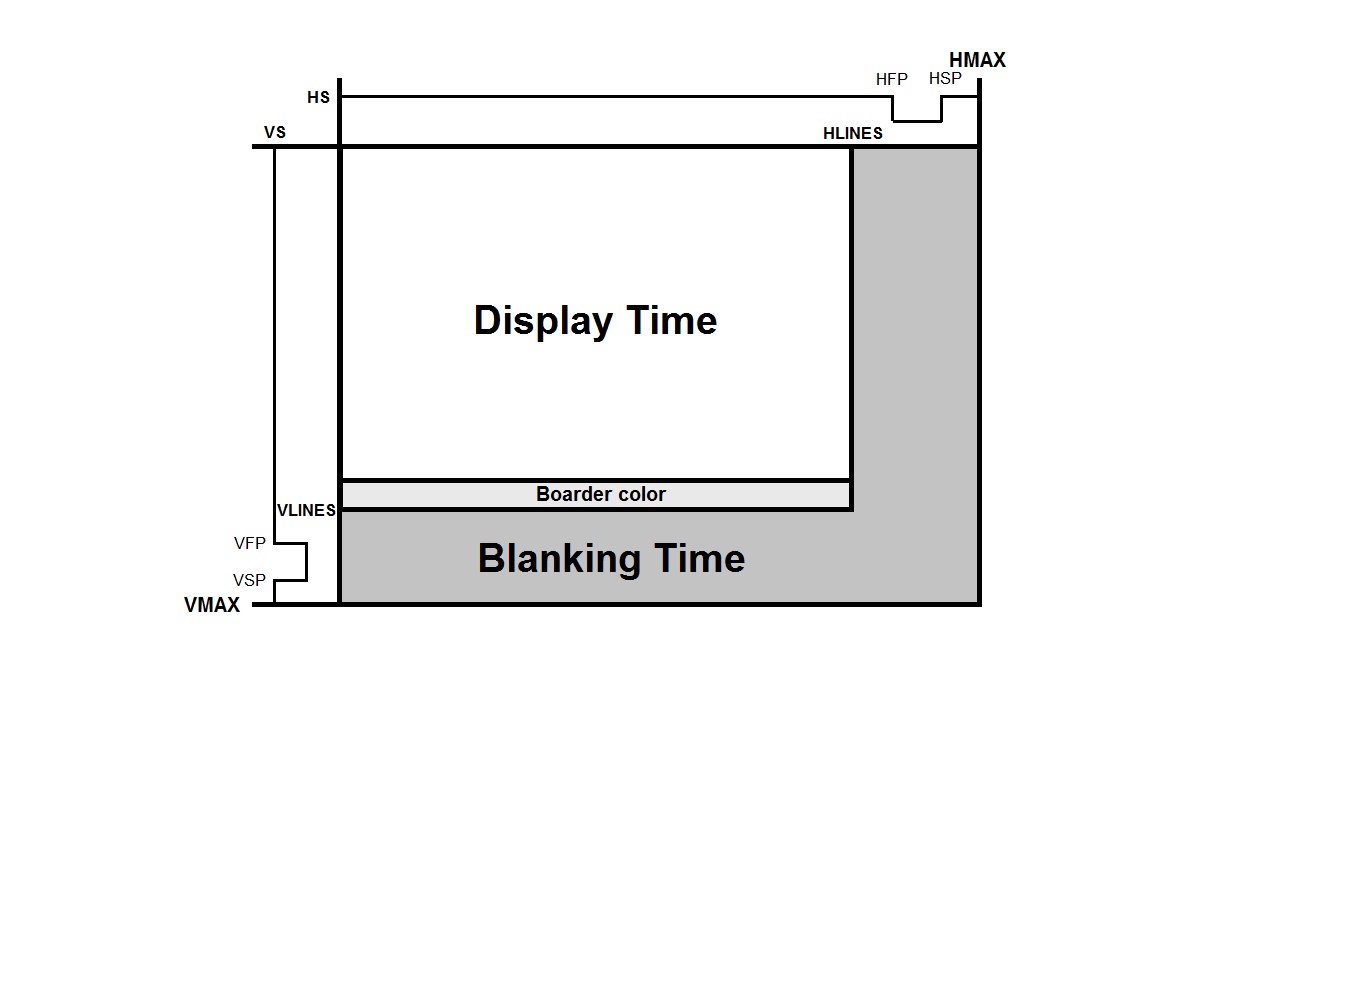
\includegraphics[width=14cm]{vga_teori.eps}
        \caption{VGA teori}
        \label{fig:vga_teori}
    \end{center}
\end{figure}

När VGA skickar pixeldata till VGA porten kommer skärmen inte ta emot och visa pixel data under hela tiden. Dessutom finns det en speciell timing till olika upplösningar med olika frekvenser. Upplösning 640x480 med frekvens 60Hz har vi följande timing enligt Digilent®.

\begin{itemize}
    \item HMAX: 800
    \item VMAX: 525
    \item HLINES: 640
    \item VLINES: 480
    \item HFP: 648
    \item HSP: 744
    \item VFP: 482
    \item VSP: 484
    \item Clk: 25MHz
\end{itemize}

Vi har blanking time för att en skärm använder en stråle för att visa varje pixel och strålen flyttar sig från vänster till höger och sedan ner på nästa rad och upprepar denna process. Under blanking time kommer strålen flytta sig från höger till vänster och under denna tid ska skärmen inte visar någon pixel. Mellan front porch och back porch går sync signal ner och upp igen på grund av att det är sync signal som uppdaterar och bestämmer frekvens till skärmen.

På display ytan, kommer varje pixel uppdateras enligt den 8 bitars färg som skärmen har fått genom VGA porten och på blank ytan ska vga porten får ingen färg data alls, annars kommer skärmen visa denna färg när de flyttar sig tillbaka över skärmen.

\subsection{RS232}

Vårt FPGA kort har en USB till RS232 port. Vi använde denna för att föra över den assemblerade spelarkoden till kortet. En överförning inleds av en startbit, därefter följer 8 databitar och en stoppbit. Hastigheten mäts i baud, tecken (på 8 bitar) per sekund. I vårt fall var ledningen hög när ingen överförning var igång (1). Överförningen inleds med att ledningen jordas (2), därefter följer 8 databitar i vald hastighet (3). I slutet av överförningen kommer en stoppbit som är hög (4). Se figur \ref{fig:rs232}.

\begin{figure}[h]
    \begin{center}
        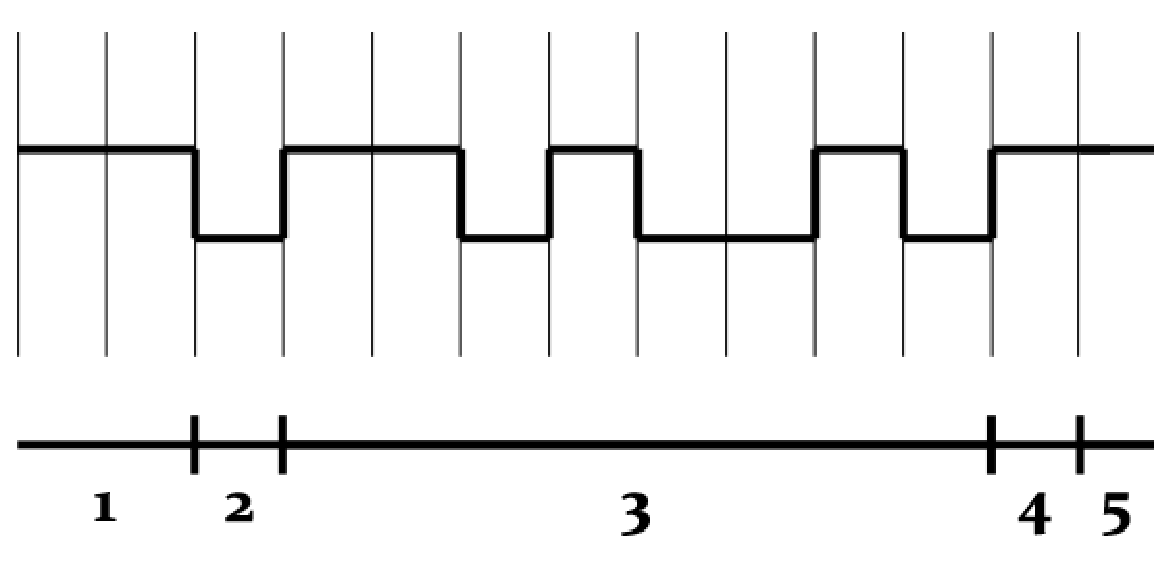
\includegraphics[width=10cm]{rs232.eps}
        \caption{En RS232 överförning. Man har ingen gemensam klocka för sändare och mottagare utan överför endast data, sändaren och mottagaren känner dock till vilken baud rate man överför med. I vårt fall använder vi 115 200 baud.}
        \label{fig:rs232}
    \end{center}
\end{figure}


\end{document}

